%
%  Vincent Yannello
%
\documentclass[12pt,fullpage]{article}
\usepackage{fullpage}
\usepackage{psfrag}                                          % LaTeX graphics tool
\usepackage{pslatex}                                         % avoids the default cmr font
\usepackage{graphicx}                                        % graphics package 
\usepackage{epsfig}                                          % figures
\usepackage{hyperref}
\usepackage{color}

\begin{document}

\noindent
{\bf Zipf distribution} (from \color{blue}\url{http://www.math.wm.edu/~leemis/chart/UDR/UDR.html}\color{black})

\noindent
The shorthand $X \sim {\rm Zipf}(\alpha, n)$ is used to indicate that the
random variable $X$ has the Zipf distribution with parameters $\alpha$ and $n$.
A Zipf random variable $X$ with parameters $\alpha$ and $n$ has probability mass function 
$$
f(x) = {\frac {1}{{x} ^ {\kern 0.08 em\alpha}\sum _{i \kern 0.04 em =1}^{n} \left(1/i
 \right) ^ {\alpha}}} \qquad \qquad x = 1, 2, \ldots, n,
$$
for all positive integers $n$ and all $\alpha \geq 0$.
The Zipf distribution can be used to account for the relative popularity of
a few members of a population and the relative obscurity of other members 
of a population.  Examples include the following.
\begin{itemize}
\item There are a few websites that get lots of hits, a greater number of websites that get a 
moderate number of hits, and a vast number of websites that hardly get any hits at all (like this one).
\item A library has a few books that everyone wants to borrow (best sellers),
a greater number of books that get borrowed occasionally (classics), and a vast number of books that
hardly ever get borrowed.
\item A natural language has a few words that are used with high frequency
(``the'' and ``of'' rank first and second in English), a greater number of words that
get used with lower frequency (like ``butter'' and ``joke''), and a vast number of words that hardly
ever get used at all (like
%  ``hippopotomonstrosesquippedalio'' which means fear of long words or
``defenestrate'' which means to throw out of a window,
%  ``abacinate'' which means to blind by putting a hot copper basin near someone's eyes,
%  ``miasma'' which means foul vapours emitted from rotting matter,
%  ``mumpsimus'' which is a view stubbornly held even when shown to be wrong,
%  ``widdershins'' which means counterclockwise,
%  ``scurryfunge'' which means a hasty tidying of your house between the time you see a neighbor and the time they knock,
``lucubration'' which means a study or composition lasting late into the night,
or ``mascaron'' which means a grotesque face on a door-knocker).
\item  The world population lives in several large cities, a greater number of medium-sized cities,
and a vast number of small towns.
\end{itemize}
The probability mass function for $\alpha = 1$ and $n = 10$ is illustrated below.

\begin{figure}[h!]
\begin{center}
\psfrag{labx}{$x$}
\psfrag{labf}{$f(x)$}
\includegraphics[width=3.6in]{ZipfPlot.ps}
\end{center}
\end{figure}

\noindent
Many times, the summation in the denominator is represented as
$$
H_{n,\alpha} = \sum _{i=1}^{n} \left( \frac{1}{i}\right) ^{\kern -0.10 em \alpha}
$$
An alternative representation is 
$$
f(x) = {\frac {1}{{x}^{\kern 0.08 em \alpha}H_{n,\alpha}}} \qquad \qquad x = 1, 2, \ldots, n.
$$
Using this shorthand notation, the cumulative distribution function on
the support of $X$ is
$$
F(x) = P(X \le x) = \frac{H_{x, \alpha}}{H_{n, \alpha}}  \qquad \qquad x = 1, 2, \ldots, n.
$$
The survivor function on the support of $X$ is
$$
S(x) = P(X \ge x) = \frac{x^{\alpha} H_{n, \alpha} - x^{\alpha} H_{x, \alpha} + 1}{x^{\alpha}H_{n, \alpha}}  \qquad \qquad x = 1, 2, \ldots, n.
$$
The hazard function on the support of $X$ is
$$
h(x) = \frac{f(x)}{S(x)} = \frac{1}{x^{\alpha}H_{n,\alpha} - x^{\alpha}H_{x,\alpha} + 1} \qquad \qquad x = 1, 2, \ldots, n.
$$
The cumulative hazard function on the support of $X$ is
$$
H(x) = - \ln S(x) = \ln \left(x^{\alpha} H_{n,\alpha}\right) - \ln \left(x^{\alpha}H_{n,\alpha} - x^{\alpha}H_{x,\alpha} + 1\right)  \qquad \qquad x = 1, 2, \ldots, n.
$$
The moment generating function of $X$ is
$$
M(t) = E\left[ e ^ {tX} \right] = \frac{1}{H_{n, \alpha}}\sum_{j=1}^n \frac{e^{jt}}{j^{\alpha}} \qquad \qquad -\infty < t < \infty.
$$
The characteristic function of $X$ is
$$
\phi(t) = E\left[ e ^ {itX} \right] =  \frac{1}{H_{n, \alpha}}\sum_{j=1}^n \frac{e^{\kern 0.04 em ijt}}{j^{\alpha}} \qquad \qquad -\infty < t < \infty.
$$
The population mean, variance, skewness, and kurtosis of $X$ are
$$
E[X] = \frac{H_{n, \alpha - 1}}{H_{n, \alpha}} \qquad \qquad
V[X] = \frac{H_{n, \alpha - 2} H_{n, \alpha} - H_{n, \alpha - 1}^2}{H_{n,\alpha}^2} \qquad \qquad 
$$
$$
E\left[ \left( \frac{X - \mu}{\sigma} \right) ^ 3 \right] = \frac{\frac{H_{n, \alpha - 3}}{H_{n, \alpha}} - 3\frac{H_{n, \alpha - 1}H_{n, \alpha - 2}}
{H_{n, \alpha}^2} + 2\frac{H_{n, \alpha - 1}^3}{H_{n, \alpha}^3}}{\left(\frac{H_{n, \alpha - 2}H_{n, \alpha} - H_{n, \alpha - 1}^2}{H_{n,
\alpha}^2} \right)
^{3/2}} \qquad \qquad 
$$
$$
E\left[ \left( \frac{X - \mu}{\sigma} \right) ^ 4 \right] = \frac{H_{n, \alpha}^3H_{n, \alpha-4} - 4H_{n, \alpha}^2H_{n, \alpha - 1}H_{n, \alpha - 3} + 6H_{n, \alpha}
H_{n, \alpha -1}^2H_{n, \alpha - 2} - 3H_{n, \alpha - 1}^4}{(H_{n, \alpha - 2}H_{n, \alpha} - H_{n, \alpha - 1}^2)^2}.
$$

\newpage

%  \vspace{0.1in}

\noindent
{\bf APPL verification:}
The APPL statements
\begin{verbatim}
assume(alpha >= 0)
X:=[[x -> 1/(x^alpha * sum((1/i)^alpha,i=1..n))], [1..n], ["Discrete", "PDF"]];
CDF(X);
SF(X);
HF(X);
CHF(X);
MGF(X);
Mean(X);
Variance(X);
Skewness(X);
Kurtosis(X);
\end{verbatim}
verify the cumulative distribution, survivor function, hazard function, cumulative hazard function, moment generating function, population mean, variance, skewness, kurtosis.
\end{document}
